\chapter{Background Knowledge and Related Work}
\label{sec:background}

This chapter provides an overview of key concepts and research that are relevant for the development of the thesis. The goal is to integrate the proposed approaches into the broader context of existing work and demonstrate how they contribute to the current state of research.

\section{Embeddings}
\label{sec:background:embeddings}
Embeddings form the foundation of many modern \ac{nlp} systems by providing a mathematical representation of words or texts in a continuous vector space. These representations capture semantic relationships, enabling machines to better understand and process human language. This section provides an overview of the evolution of embedding techniques, from early static word vectors to more recent context-aware models, and highlights their importance in a wide range of \ac{nlp} applications.

\begin{figure}[ht]
  \begin{center}
    % source: https://www.cs.cmu.edu/~dst/WordEmbeddingDemo/tutorial.html
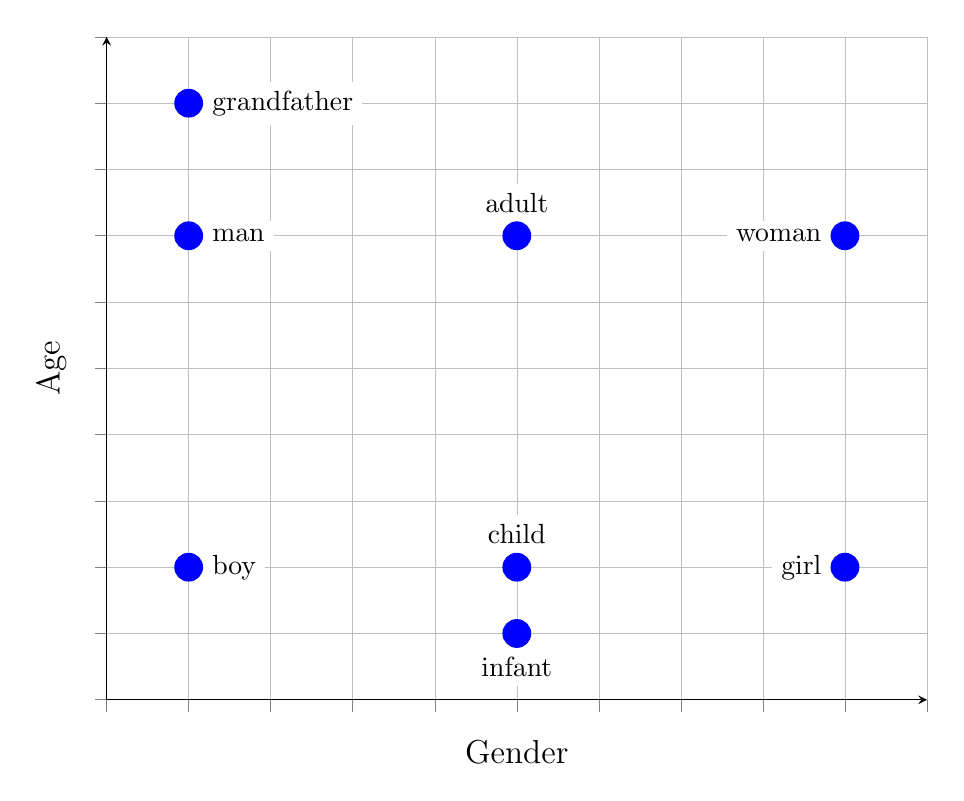
\begin{tikzpicture}
  \begin{axis}[
      width=12cm, height=10cm,
      xlabel={Gender}, ylabel={Age},
      xmin=0, xmax=10, ymin=0, ymax=10,
      xtick={0,1,...,10}, ytick={0,1,...,10},
      xticklabel={\empty}, yticklabel={\empty},
      grid=both,
      grid style={line width=.1pt, draw=gray!30},
      major grid style={line width=.2pt,draw=gray!50},
      axis lines=left,
      tick align=outside,
      enlargelimits=false,
      label style={font=\large},
      title style={font=\LARGE, yshift=1em},
      every tick label/.append style={font=\small},
    ]

    % Plot the points
    \addplot[
      only marks,
      mark=*,
      mark size=5pt,
      blue,
    ] coordinates {
        (1,9)   % grandfather
        (1,7)   % man
        (1,2)   % boy
        (5,7)   % adult
        (5,2)   % child
        (5,1)   % infant
        (9,7)   % woman
        (9,2)   % girl
      };

    % Add labels
    \node[fill=white, anchor=west, xshift=5pt, font=\normalsize] at (axis cs:1,9)  {grandfather};
    \node[fill=white, anchor=west, xshift=5pt, font=\normalsize] at (axis cs:1,7)  {man};
    \node[fill=white, anchor=west, xshift=5pt, font=\normalsize] at (axis cs:1,2)  {boy};
    \node[fill=white, anchor=south, yshift=5pt, font=\normalsize] at (axis cs:5,7)  {adult};
    \node[fill=white, anchor=south, yshift=5pt, font=\normalsize] at (axis cs:5,2)  {child};
    \node[fill=white, anchor=north, yshift=-5pt, font=\normalsize] at (axis cs:5,1)  {infant};
    \node[fill=white, anchor=east, xshift=-5pt, font=\normalsize] at (axis cs:9,7)  {woman};
    \node[fill=white, anchor=east, xshift=-5pt, font=\normalsize] at (axis cs:9,2)  {girl};
  \end{axis}
\end{tikzpicture}
  \end{center}
  \caption{TODO:}
  \label{fig:embeddings} % TODO: reference
\end{figure}

Early models for word representation focused on learning fixed vectors for each word, resulting in what are known as static word embeddings. These embeddings assign the same vector to a word regardless of the context in which it appears. Well-known examples of such approaches include Word2Vec \cite{mikolovEfficientEstimationWord2013} and GloVe \cite{penningtonGloveGlobalVectors2014}, both of which capture semantic similarities based on word co-occurrence statistics in large text corpora.

While static embeddings are computationally efficient and useful in many scenarios, they are unable to account for variations in word meaning across different contexts. This limitation has led to the development of models that produce context-dependent embeddings, referred to as contextual word embeddings. A prominent early example is ELMo \cite{petersDeepContextualizedWord2018}, which uses bidirectional LSTMs to generate embeddings that are sensitive to the surrounding words in a sentence.

More recent approaches employ transformer-based architectures. Models such as BERT \cite{devlin-etal-2019-bert} generate deep contextual embeddings by using self-attention mechanisms to model relationships between words in context. Contextual information is crucial, as it enables models to disambiguate polysemous words. For instance, the word \enquote{bank} can either refer to a financial institution or the side of a river, and only contextual clues can determine the correct meaning.

These contextual embeddings have substantially improved performance across a wide variety of \ac{nlp} tasks, including question answering, named entity recognition, and machine translation. Consequently, they have become foundational components in modern \ac{nlp} pipelines.

\section{Stylistic Investigations}
\label{sec:background:styleInvestigations}
% TODO: write a little more about the proxy tasks; what are they, what are examples, why are they necessary
% TODO: example for learned style embedding method with citation
Stylometric analysis is concerned with capturing an author's writing style in a way that is independent of the actual content being conveyed. Modern neural approaches often achieve this by learning dense vector representations, or style embeddings, through the use of proxy tasks. These tasks include style transfer, authorship attribution or verification, and group membership detection. Proxy tasks allow models to learn stylistic features without the need for explicit style annotations.

However, one drawback of learned style embeddings is that it is difficult to ensure that the representations are truly independent of the content. % TODO: citation?
This complicates their application in new domains. Another disadvantage is that such embeddings tend to be uninterpretable, which reduces their transparency and limits their usefulness in downstream tasks.

To address these issues, some approaches aim to produce interpretable embeddings. Notable examples include the work by \citet{patelLearningInterpretableStyle2023}, who propose a method for learning attribute-based representations, and \citet{alshomaryLatentSpaceInterpretation2024}, who focus on interpreting latent embeddings. The thesis builds on and extends this line of research by proposing a new method to learn interpretable style embeddings that also incorporate knowledge-related dimensions.

Classical methods for stylistic analysis take a different approach by manually selecting interpretable features such as frequencies of function words, syntactic structures, or punctuation counts. % TODO: citation and/or short explanations what the examples are
These handcrafted features can be used to construct explainable classifiers, although they may lack the nuance and representational capacity of neural embeddings.

One example of recent work in this area is Stylometrix by \citet{okulskaStyloMetrixOpensourceMultilingual2023}, which generates interpretable style vectors based on a curated set of features. Another is StyloAI by \citet{oparaStyloAIDistinguishingAIgenerated2024a}, which extracts \num{31} stylometric features to identify AI-generated texts using a Random Forest classifier.

The main advantages of such feature-based approaches are the high relevance and quality of the extracted features. However, these methods also have several drawbacks. They require manual selection of features, which limits the range of stylistic attributes that can be captured. Moreover, they cannot incorporate more abstract attributes that require a deeper understanding of the text, such as the knowledge-related features used in this thesis.

\section{Large Language Models}
\label{sec:background:llm}

Large Language Models (\acfp{llm}) are large-scale neural networks with typically billions of parameters. These models are pre-trained on massive corpora of text and are capable of performing tasks that require advanced language understanding and generation \cite{minaeeLargeLanguageModels2025}.

\acp{llm} have brought significant advancements to the field of \ac{nlp}, achieving state-of-the-art performance in a broad range of applications. These include text generation, translation, and question answering, among many others.

The architecture that underpins most modern \acp{llm} is the transformer, introduced by \citet{NIPS2017_3f5ee243} in the seminal paper \textit{Attention Is All You Need}. In contrast to earlier models that relied on recurrence or convolution, the transformer architecture employs self-attention mechanisms that allow the model to weigh the relevance of each word in the input sequence relative to others. This design supports parallel processing, thereby improving training efficiency and scalability.

The transformer follows an encoder-decoder architecture, illustrated in Figure~\ref{fig:transformerArchitecture}. The encoder processes the input sequence and produces a continuous representation, while the decoder generates the output sequence conditioned on both the encoder's output and its own previous outputs.

In this thesis, encoder-only \acp{llm} will be employed for the creation of interpretable attribute embeddings. Decoder-only \acp{llm} will be used for the task of text generation.

\begin{figure}[ht]
  \begin{center}
    \input{figures/tikz/transformer-architecture.tex}
  \end{center}
  \caption{TODO:} % TODO: mention source (attention is all you need); explain layers
  % source: https://www.cs.cmu.edu/~dst/WordEmbeddingDemo/tutorial.html
  \label{fig:transformerArchitecture}
\end{figure}

\section{Steering of Large Language Models}
\label{sec:background:llm:steering}

While \acp{llm} are highly effective at generating coherent and fluent text, it is often desirable to guide the generated text to follow specific constraints or stylistic forms. It is also critical to ensure that models avoid generating toxic or inappropriate content. Several steering methods have been developed to address these challenges.

One widely used method is \textbf{prompt engineering}, which steers the model by modifying the input prompt provided during inference. This approach has the key advantage that it does not require any model training \cite{schulhoffPromptReportSystematic2024}.

Prompt engineering comes in several variations. One important type is the system prompt, which is particularly relevant in chat-based \acp{llm}. The system prompt defines the model's behavior and tone throughout a conversation. Although it is hidden from the user, it can influence the model to adopt a specific persona, adhere to certain formatting rules, or follow predefined safety guidelines. For example, the system prompt can instruct the model to act as a helpful tutor, or to avoid discussing certain topics.

Another variant of prompt engineering is few-shot prompting. In this approach, the prompt not only contains instructions for the task, but also includes a few examples of correct task completions. These examples enable the model to generalize to similar tasks based on the provided patterns.

% chain-of-thought prompting by Wei et al., 2022 % TODO: include this?

A more resource-intensive method of steering is \textbf{fine-tuning}, which involves updating the model's parameters on task-specific data. Although fine-tuning can yield strong performance, it is often prohibitively expensive for \acp{llm} due to their size. Additionally, deploying a separate fine-tuned model for each task can be inefficient and impractical.

To mitigate these issues, parameter-efficient fine-tuning methods have been proposed. These methods freeze the pre-trained model weights and train only a small number of additional parameters. One such method is prefix-tuning \cite{liPrefixtuningOptimizingContinuous2021}, where a learned vector (prefix) is prepended to the model input, achieving competitive performance while training only \SI{0.1}{\percent} of the model's parameters. Another example is LoRA \cite{huLoRALowrankAdaptation2021}, which introduces trainable low-rank matrices into the model while keeping the original weights fixed. LoRA reduces the number of trainable parameters by a factor of \num{10000} without compromising performance.

% \textbf{Reinforcement Learning from Human Feedback (RLHF)} % TODO: include this?

A recent alternative to these methods is \textbf{activation steering}. This technique works by directly modifying the hidden states of a \ac{llm} during inference to influence the output. Hidden states are typically extracted at the end of each transformer layer, and state-of-the-art \acp{llm} can have between \num{20} and \num{100} layers. The later layers tend to capture more abstract and complex concepts \cite{bogdanEmergentEffectsScaling2025}.

Activation steering involves identifying and extracting the hidden states that correspond to specific concepts in a single forward pass. These extracted vectors, known as steering vectors, are then added to the model's internal states during inference to guide the generation process in a desired direction \cite{konenStyleVectorsSteering2024,turnerActivationAdditionSteering2024,subramaniExtractingLatentSteering2022}.
